\documentclass[11pt,twocolumn,letterpaper]{article}
\usepackage[english]{babel}
\usepackage{cvpr}
\usepackage{times}
\usepackage{epsfig}
\usepackage{graphicx}
\graphicspath{{images/}}
\usepackage{amsmath}
\usepackage{amssymb}
\usepackage{caption}
\usepackage[breaklinks=true,bookmarks=false]{hyperref}

\cvprfinalcopy

\def\httilde{\mbox{\tt\raisebox{-.5ex}{\symbol{126}}}}

\title{\LARGE FormulaTour}

\author{Gianluca Capozzi\\
	"La Sapienza" University of Rome\\
	{\tt\small capozzi.1693255@studenti.uniroma1.it}
	\and
	Marco Costa\\
	"La Sapienza" University of Rome\\
	{\tt\small costa.1691388@studenti.uniroma1.it}
}


\begin{document}
\twocolumn[{
	\renewcommand\twocolumn[1][]{#1}
	\maketitle
	\begin{center}
		\centering
		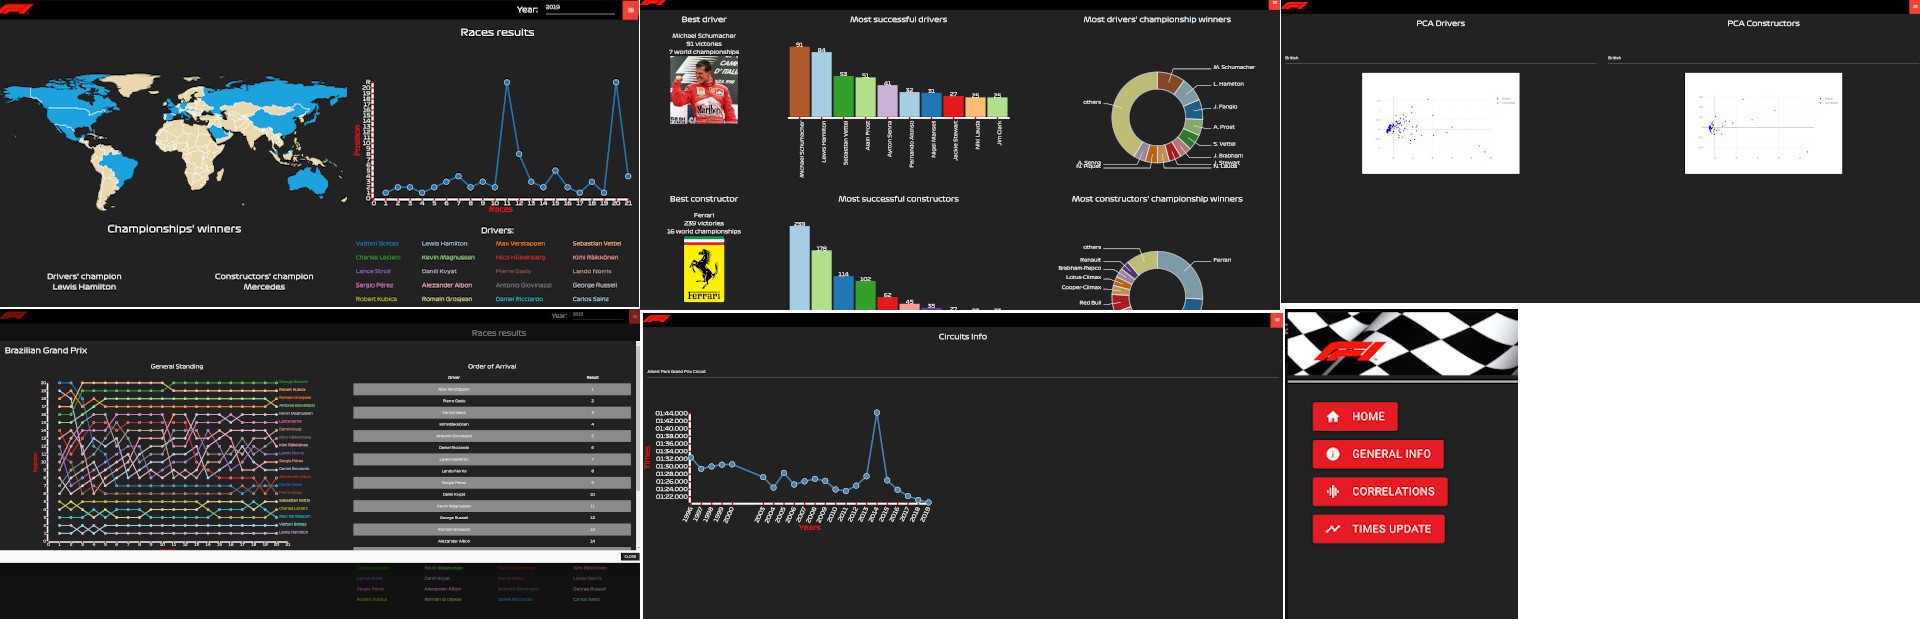
\includegraphics[width=\textwidth]{allViews}
		\captionof{figure}{Framework Views: (a) Home view, with world interactive map, winners of the season and interactive drivers trend; (b) Circuit view, with drivers standing and final ranking of the race; (c) General info view, with best driver and constructor,  most successfull drivers and constructors; (d) Correlations view, with scatter plot showing correlation between driver's or constructor's nationality and wins; (e) Circuit info view, with scatter plot showing time trend in the years for each circuit; (f) Menu}
	\end{center}
	\rule{\textwidth}{1pt} \\ \\
	\begin{abstract}
		The purpose of our application is to provide a framework able to graphically display data about Formula 1 through a user-friendly interface. It's possible to navigate through different views in order to get visual informations about this sport.
The application allows you to analyze the history of Formula 1 from the first World Championship (1950) to the last (currently 2019).
	\end{abstract}
\rule{\textwidth}{1pt}
}]

\clearpage

\section{Introduction}
Formula 1 has a very long history, as it has reached the $70^{th}$ season. During all these years many drivers and constructors took part to the races, which took place in different circuits located in different countries. This means that it is very difficult to navigate this history, since it is characterized by many components, each related to the other. The goal of this project is to provide a way to navigate the history of the Formula 1 by highlighting each component and their relations. Broadly, Formula 1 is characterized by three main elements: the drivers, the constructors and the races. These components have evolved over the years, thanks to the introduction of new technologies and regulatory changes, causing an improvement in performance. Most of these evolutions are visible in our framework, for example, it is possible to see that nowadays the number of races has increased while the lap times have reduced significantly.\\
Our framework is divided into four main views, each of which contains multiple sub-views. An initial view that summarizes the races of the selected season by showing the countries and the exact location of the circuit in which they took place together with the results. A general view that summarizes the most important results achieved by the drivers and the constructors during the Formula 1 history. A correlation view that shows if it exists a correlation between a specific nationality selected by the user and some other statistics related to drivers/constructs with that nationality. The last view is a times update view that summarizes the evolution of the lap times on a selected circuit during the years.\\
So, the framework is divided in two parts:
\begin{itemize}
	\item An analytics part that computes the examination and exploration of Formula 1 history;
	\item A visual representation of the features computed by the analytics part.
\end{itemize}
The project is a web application and it is developed using the d3.js \cite{D3} library and the Python3 language for implementing a server in order to perform some backend functionalities.

\section{Related works}
There are other frameworks that show the evolution of Formula 1 through its different elements, so races, drivers and constructors. An example is the History of F1 \cite{HistoryOfF1} framework, based on the same dataset used for this project. The main difference is that in that project there is not a division of the races with respect to the years and also the user is not able to locate geographically the position of the circuits. 

\section{Dataset}
The dataset used for this project is obtained from the Ergast Developer API \cite{Dataset}; it is available in different formats but, since both in d3.js \cite{D3} and Python3 is easy to manipulate data in .csv format, we have chosen this specific format. It is composed by 13 tables: circuits, constructorResults, constructorStandings, constructors, driverStandings, drivers, lapTimes, pitStops, qualifying, races, results, seasons and status. The tables considered for this project are:
\begin{itemize}
	\item races: a table that contains information about each race, as the year and the date in which it was run, the circuitId (which identifies the circuit in which it took place), the name of the Grand Prix (such as Italian Grand Prix) and so on;
	\item circuits: a table that contains information about each circuit, such as the name of the circuit, its coordinates, the country and so on;
	\item drivers: a table that contains information about each driver, such as his name and surname, his date of birth, his nationality and so on;
	\item results; a table that, for each race and driver who took part in that race, shows the result of that driver in that race and other infos;
	\item driverStandings: a table that, for each race and driver who took part in that race, shows the driver's points into the drivers' standing after the conclusion of that race;
	\item qualifying: a table that, for each race and driver who took part in that race, shows the results that the given driver achieves during the qualifying for that race;
	\item constructors: a table that contains information about each constructor that took part at least to one Formula 1 race;
	\item constructorStandings: a table that, for each constructor and each race, shows the results of the constructor's points into the corresponding standing after the conclusion of that race. 
\end{itemize}
The .csv files are manipulated using both d3.js and python. Some of the queries performed over the dataset needs an input from the user, while others are performed by only manipulating the original data.

\section{Design Overview}

Our framework is composed, as anticipated in the introduction, by four main views. It is possible to navigate through the application using the simple slide menu that is shown by clicking on the button on the top-right corner. This menu is composed by four buttons, each of which redirects the user to the corresponding view.
\begin{center}
	\centering
	
\includegraphics[width=0.3\columnwidth]{menu}
	\captionof{figure}{Menu}
\end{center}
In the next sections each view will be explained more in depth, analysing especially the design.

\subsection{Home view}
\begin{center}
	\centering
	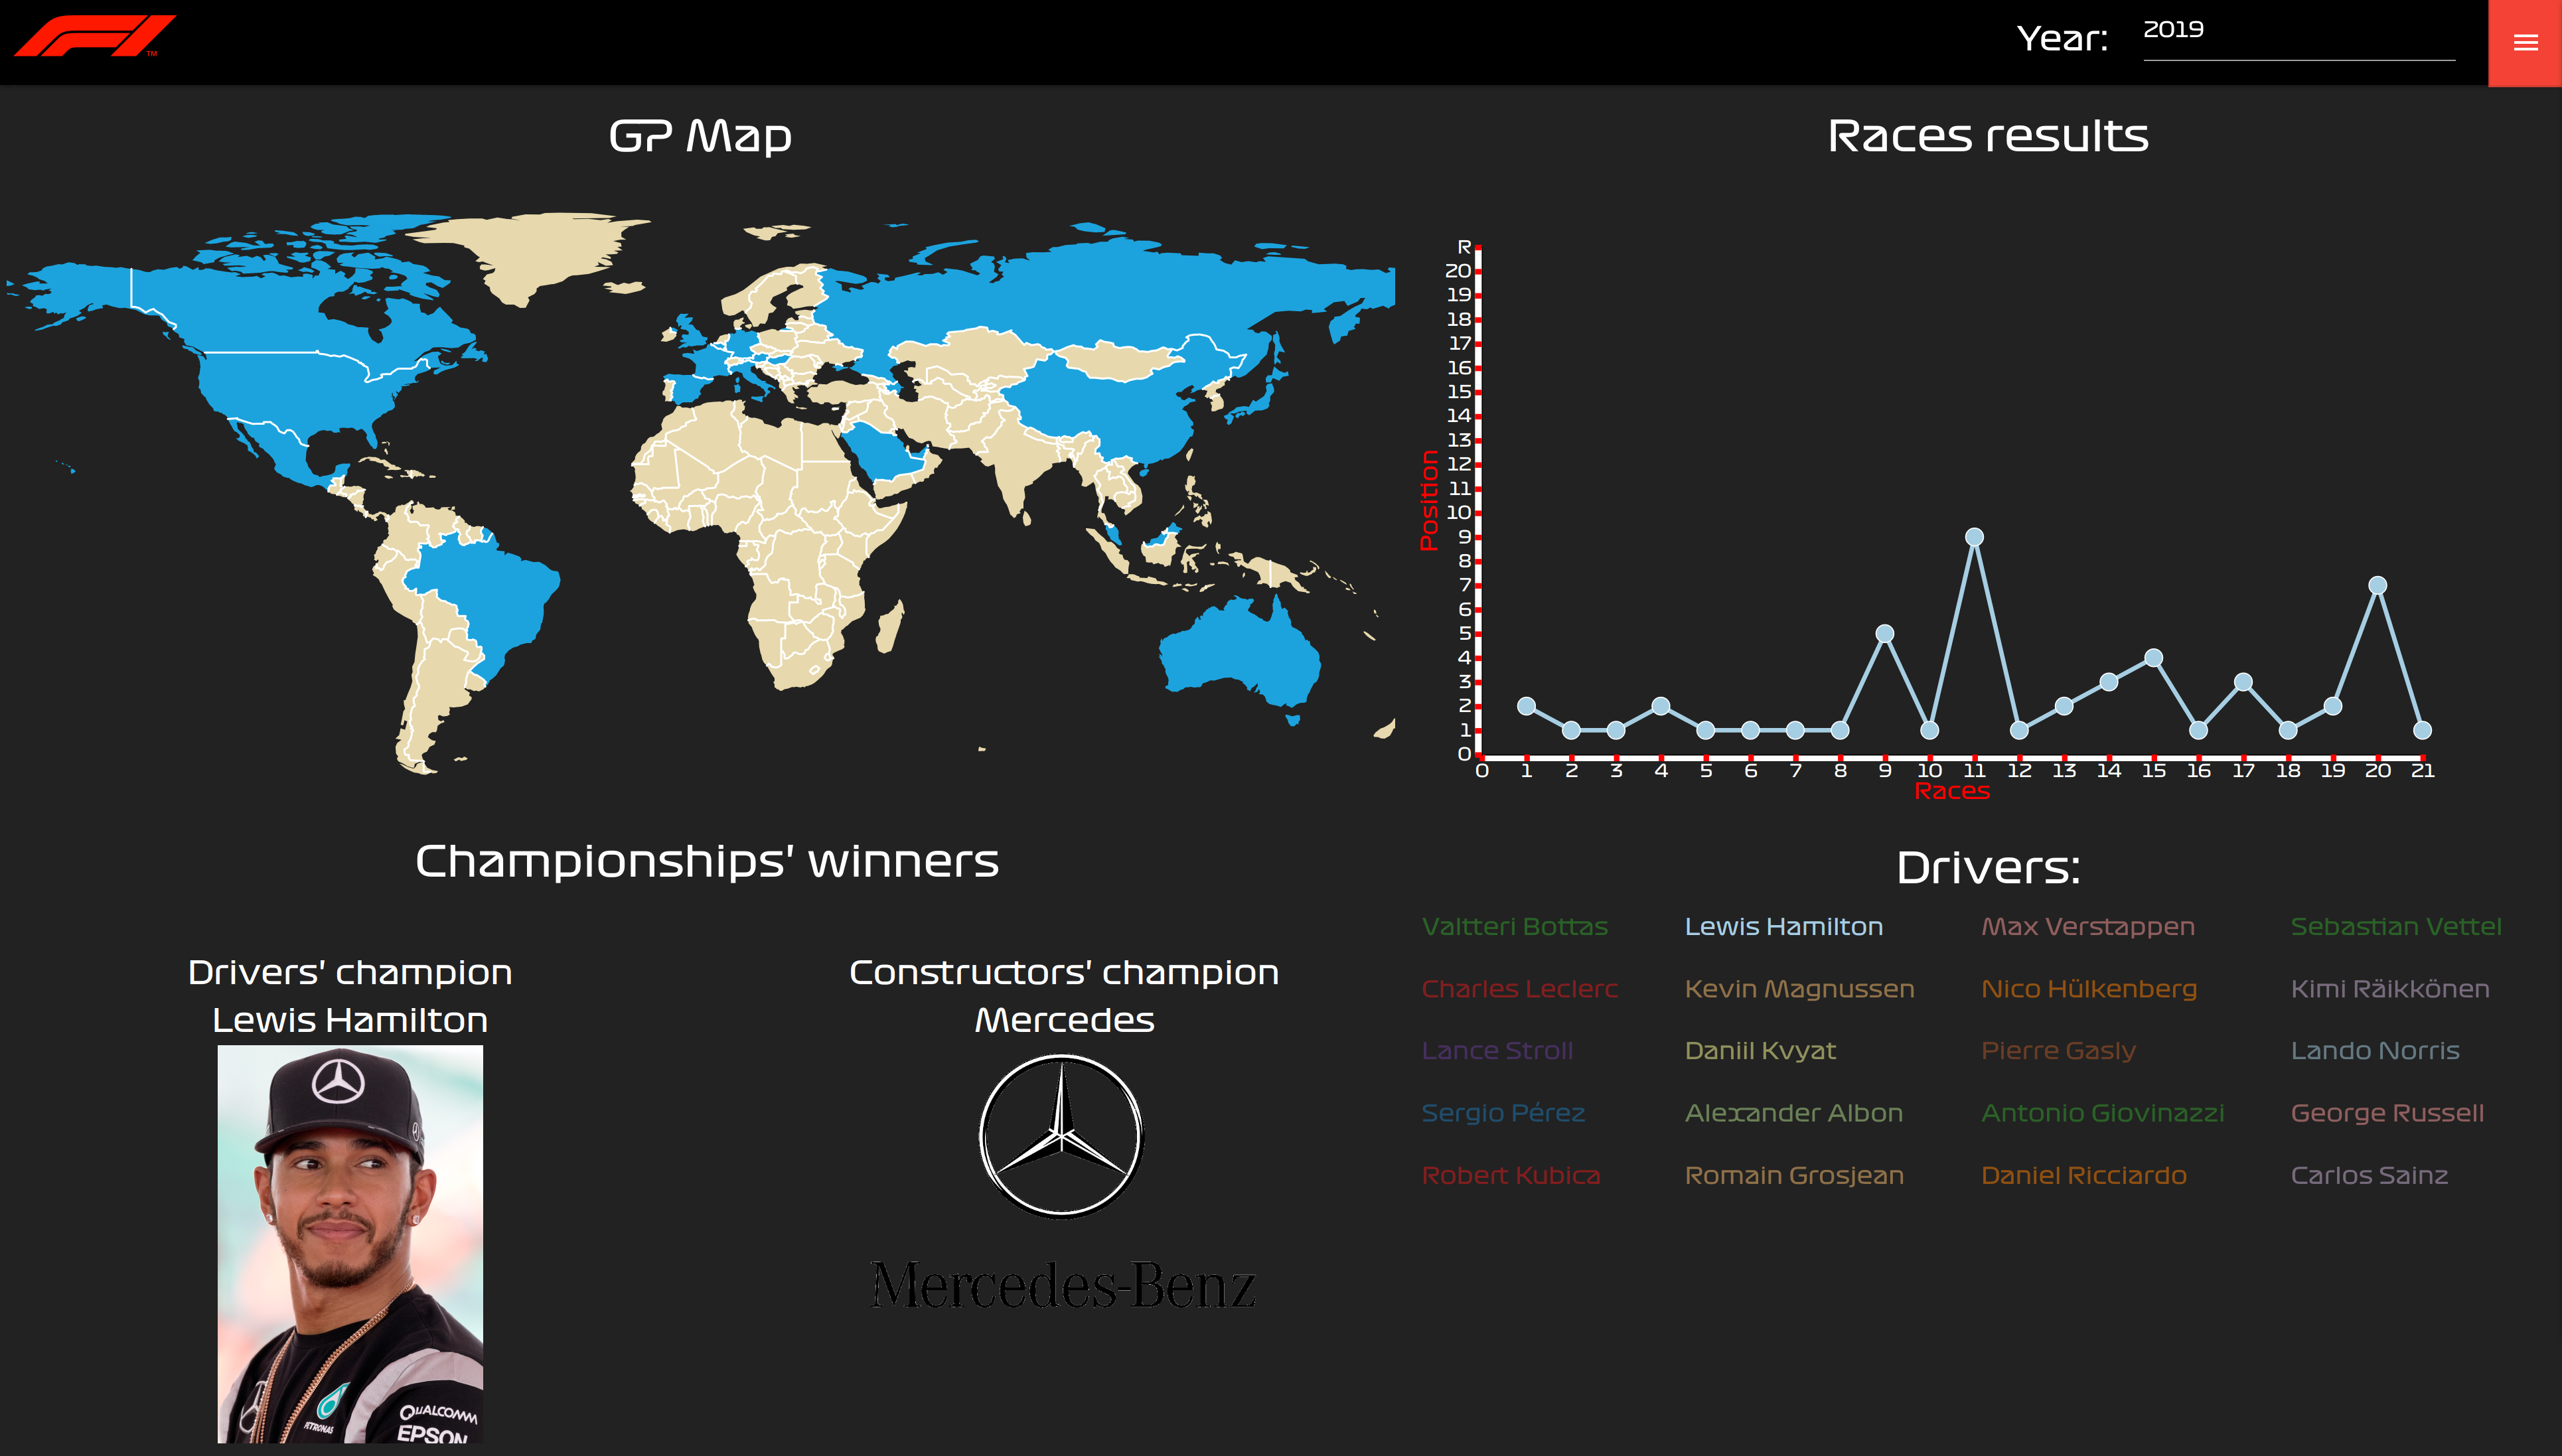
\includegraphics[width=\columnwidth]{home}
	\captionof{figure}{Home view}
\end{center}

This is the home view. Here the user is able to select the desired year from the special selector: the available years are from 1950 to 2019, so from the year in which the first F1 championship was played till the year in which the last one was played. The home view is divided into four sub-views:

\begin{itemize}
	\item a map that highlights the countries in which there was at least one Grand Prix during the selected year;
	\item a scatter plot that shows, for each driver and each race run during that year, his final position for that race;
	\item a sub-view that shows the driver and the constructor that have won the two championships at the end of the selected season;
	\item a sub-view that allows the users to selected a driver: by clicking on the name the scatter plot will be modified, showing the results of the selected driver.
\end{itemize}

The colors of the lines in the scatter plot are consistent with the colors of the name of the drivers.\\ 
The map is interactive, indeed the user can click on one of the highlighted countries (a country is colored in blue if during the selected year there was at least one Grand Prix played in that country): at this point, there will be a zoom on the selected country and a red circle showing the position of the circuit in which the race was played. By clicking on the red circle, the following view will be shown to the user:

\begin{center}
	\centering
	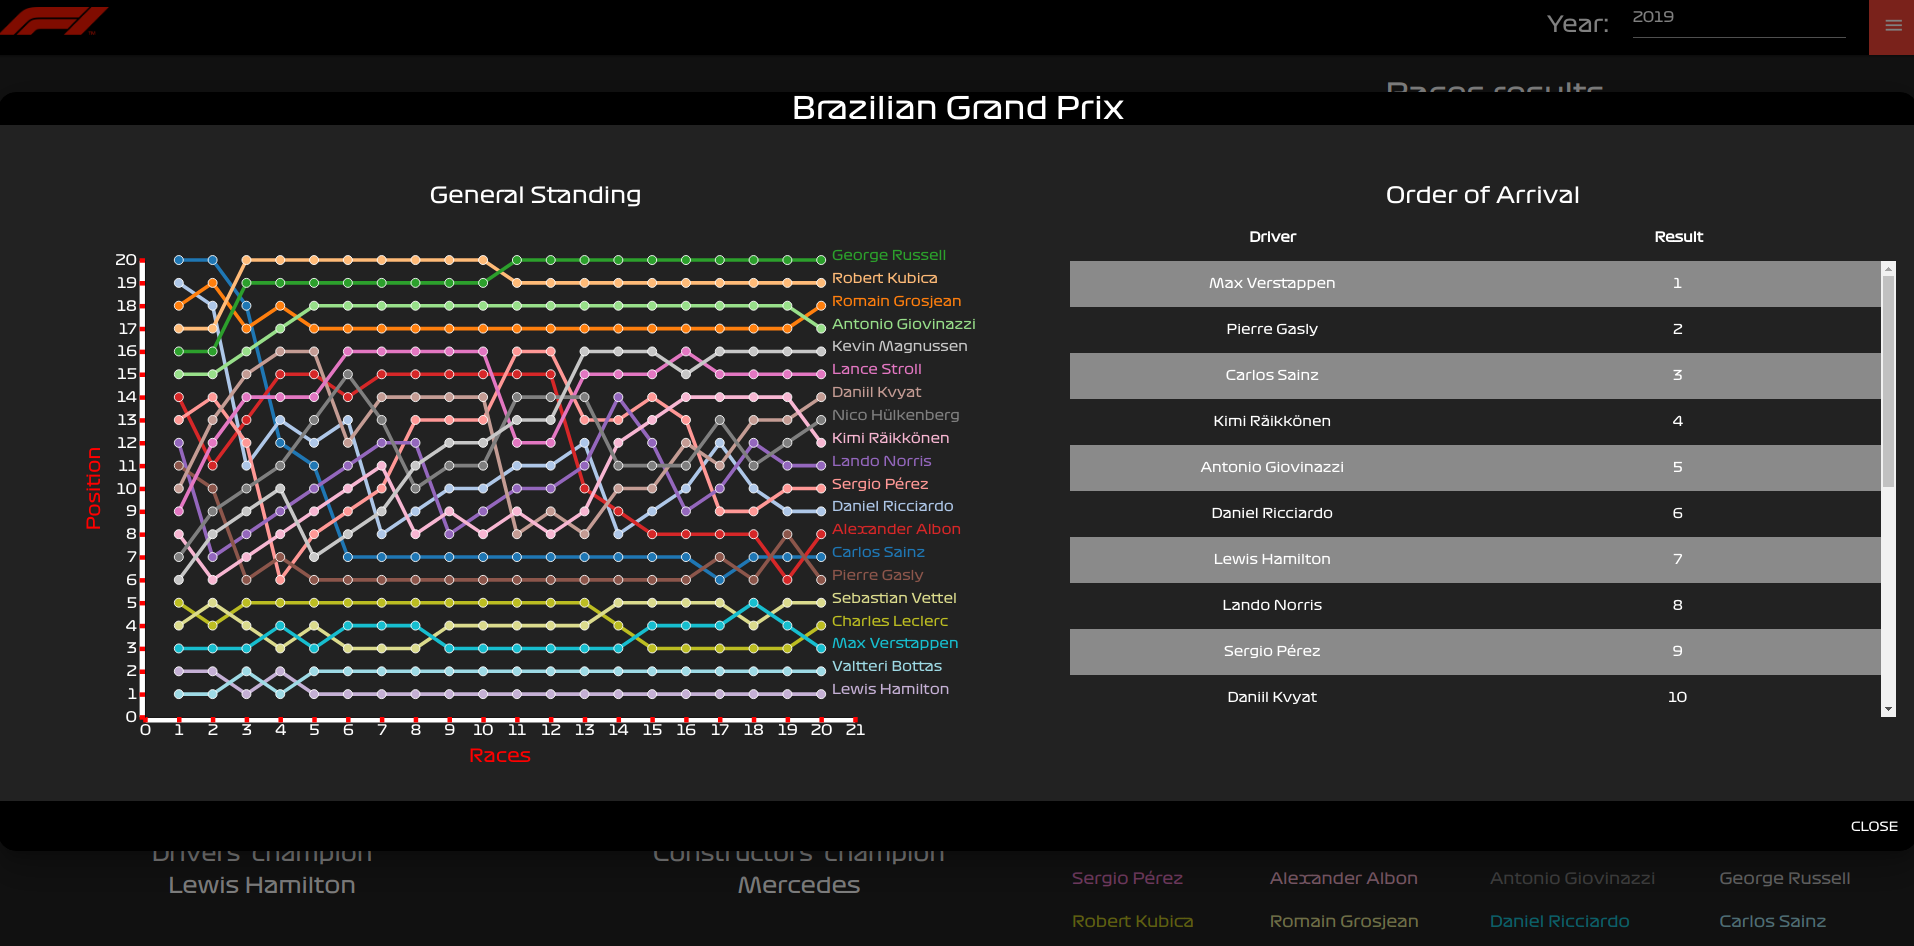
\includegraphics[width=\columnwidth]{map-clicked}
	\captionof{figure}{Race infos}
\end{center}

On the left, there is a scatter plot that shows the evolution of the drivers' standing till the selected GP; on the right, there is a table showing the order of arrival of the selected race.

\subsection{General info view}
\begin{center}
	\centering
	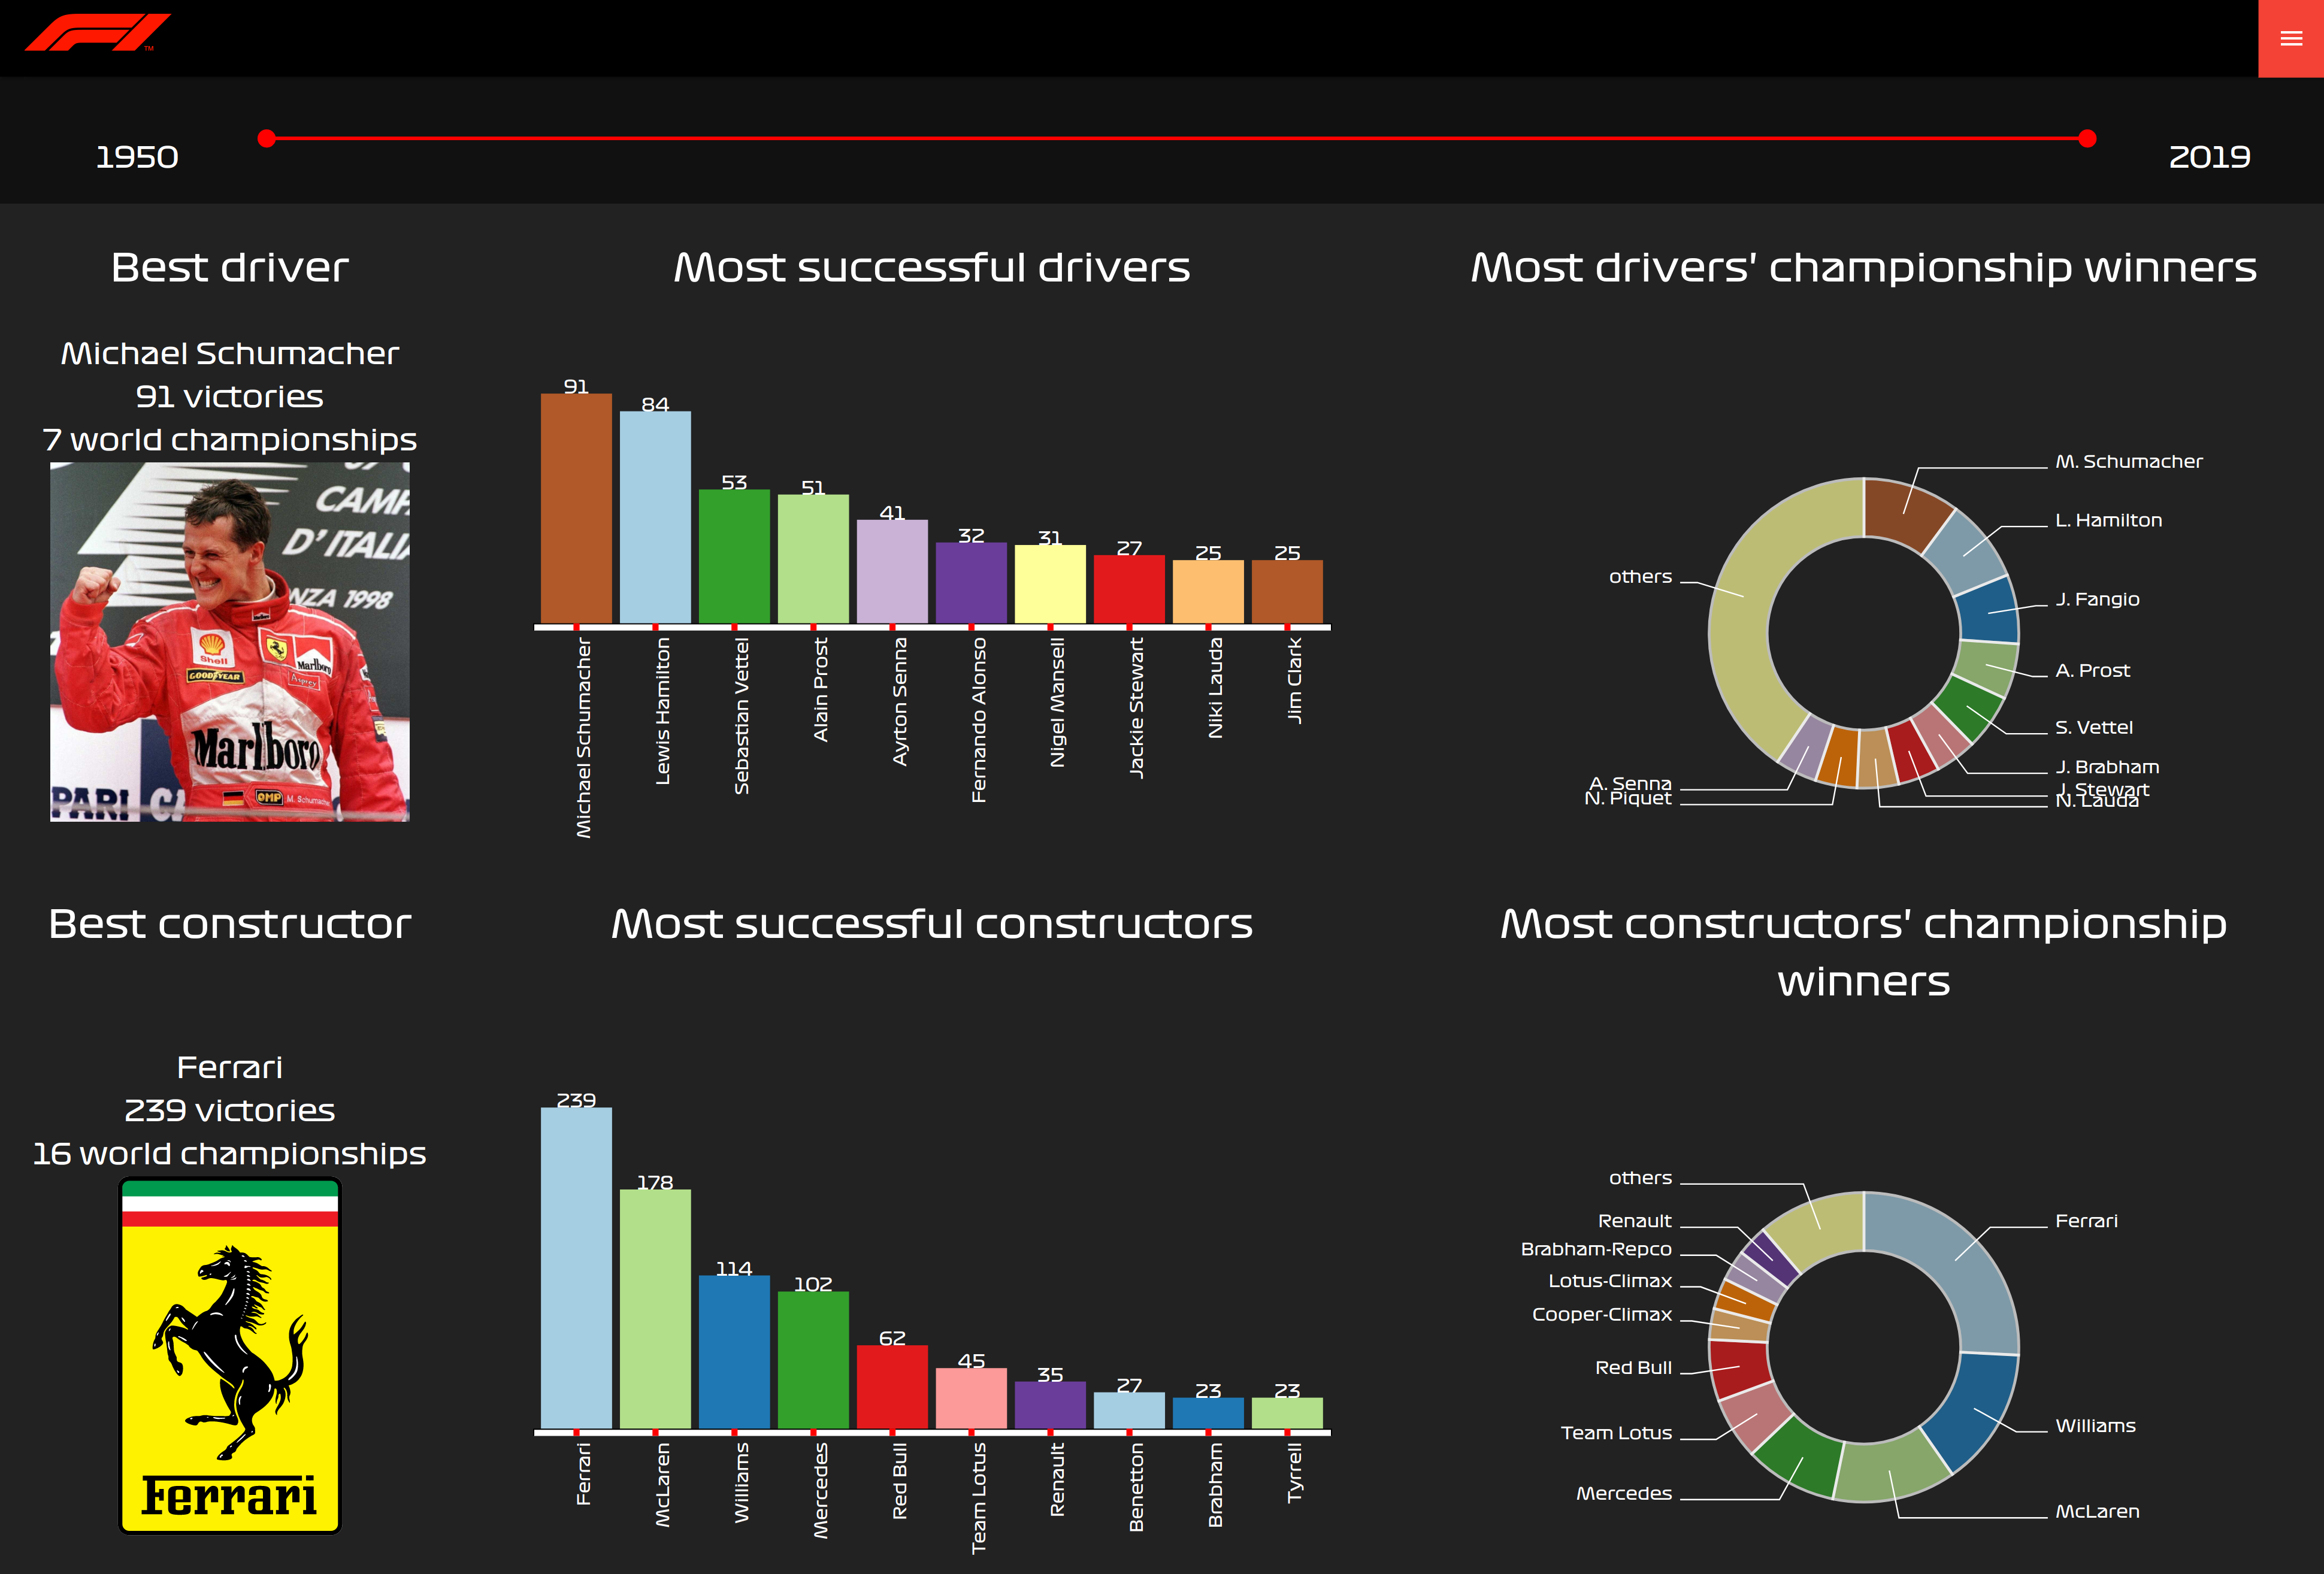
\includegraphics[width=\columnwidth]{generalinfo}
	\captionof{figure}{General info view}
\end{center}
In this view, we show some statistics about the general world of the Formula 1. It is a grid view divided in two rows and three columns: the first row highlights the drivers while the second one the constructors. The three elements of the first row describe the following statistics:
\begin{itemize}
	\item Best Driver: this is the driver that has won the most races of all the drivers. Here we show the number of victories of this driver and the number of drivers' championship that he has won;
	\item Most successful drivers: this is a top 10 based on the number of races won by a driver and it is presented using a bar chart. Each bar is associated to a driver and represents the number of races won by that driver; on top of the bar there is a number representing this statistic;
	\item Most drivers' championship winners: this is a top 10 based on the number of drivers' world titles won by a driver (we have added also the number of championships won by all the other drivers) and it is presented using a donut chart: each slice is associated to a driver and by sliding the mouse over the slice it is possible to see the number of championships won by that driver.
\end{itemize}
The two charts presented in this first row are linked together using a double interaction: by clicking on a bar of the first chart it will be highlighted together with the slice of the other chart corresponding to the same driver (if it exists). The same happens by clicking on a slice of the donut chart.\\
As said before, in the second row there are some statistics about the constructors:
\begin{itemize}
	\item Best Constructor: this is the constructor that has won the most races of all the constructors. Together with its name we show also the number of race victories and the number of constructors' world titles that it has won;
	\item Most successful constructors: this chart shows the 10 constructors that have won the most races at all. It is a bar chart where each bar refers to a constructor with on top of it the corresponding number of victories;
	\item Most constructors' championship winners: this chart shows the 10 constructors that have won more world titles: it is a donut chart where each slice is associated to a driver (we have added also a slice representing the number of world titles won by the other constructors); by sliding the mouse over the slice it is possible to see the number of championships won by that constructors.
\end{itemize}
Also in this case there is a double interaction between the two charts, similar to the one described before.\\
In both the bar charts, by sliding the mouse over a bar, it is possible to have some informations:
\begin{itemize}
	\item drivers: date of birth, nationality, teams for which it has driven, number of races that it has started and number of podiums;
	\item constructors: nationality, number of started races and number of podiums.
\end{itemize}
In both the rows there is a consistency between the colors of the bar and the slice associated to the same driver/constructor. The distribution of the different sub-views in the two rows follows a common pattern.

\newpage
\subsection{Correlations view}
\begin{center}
	\centering
	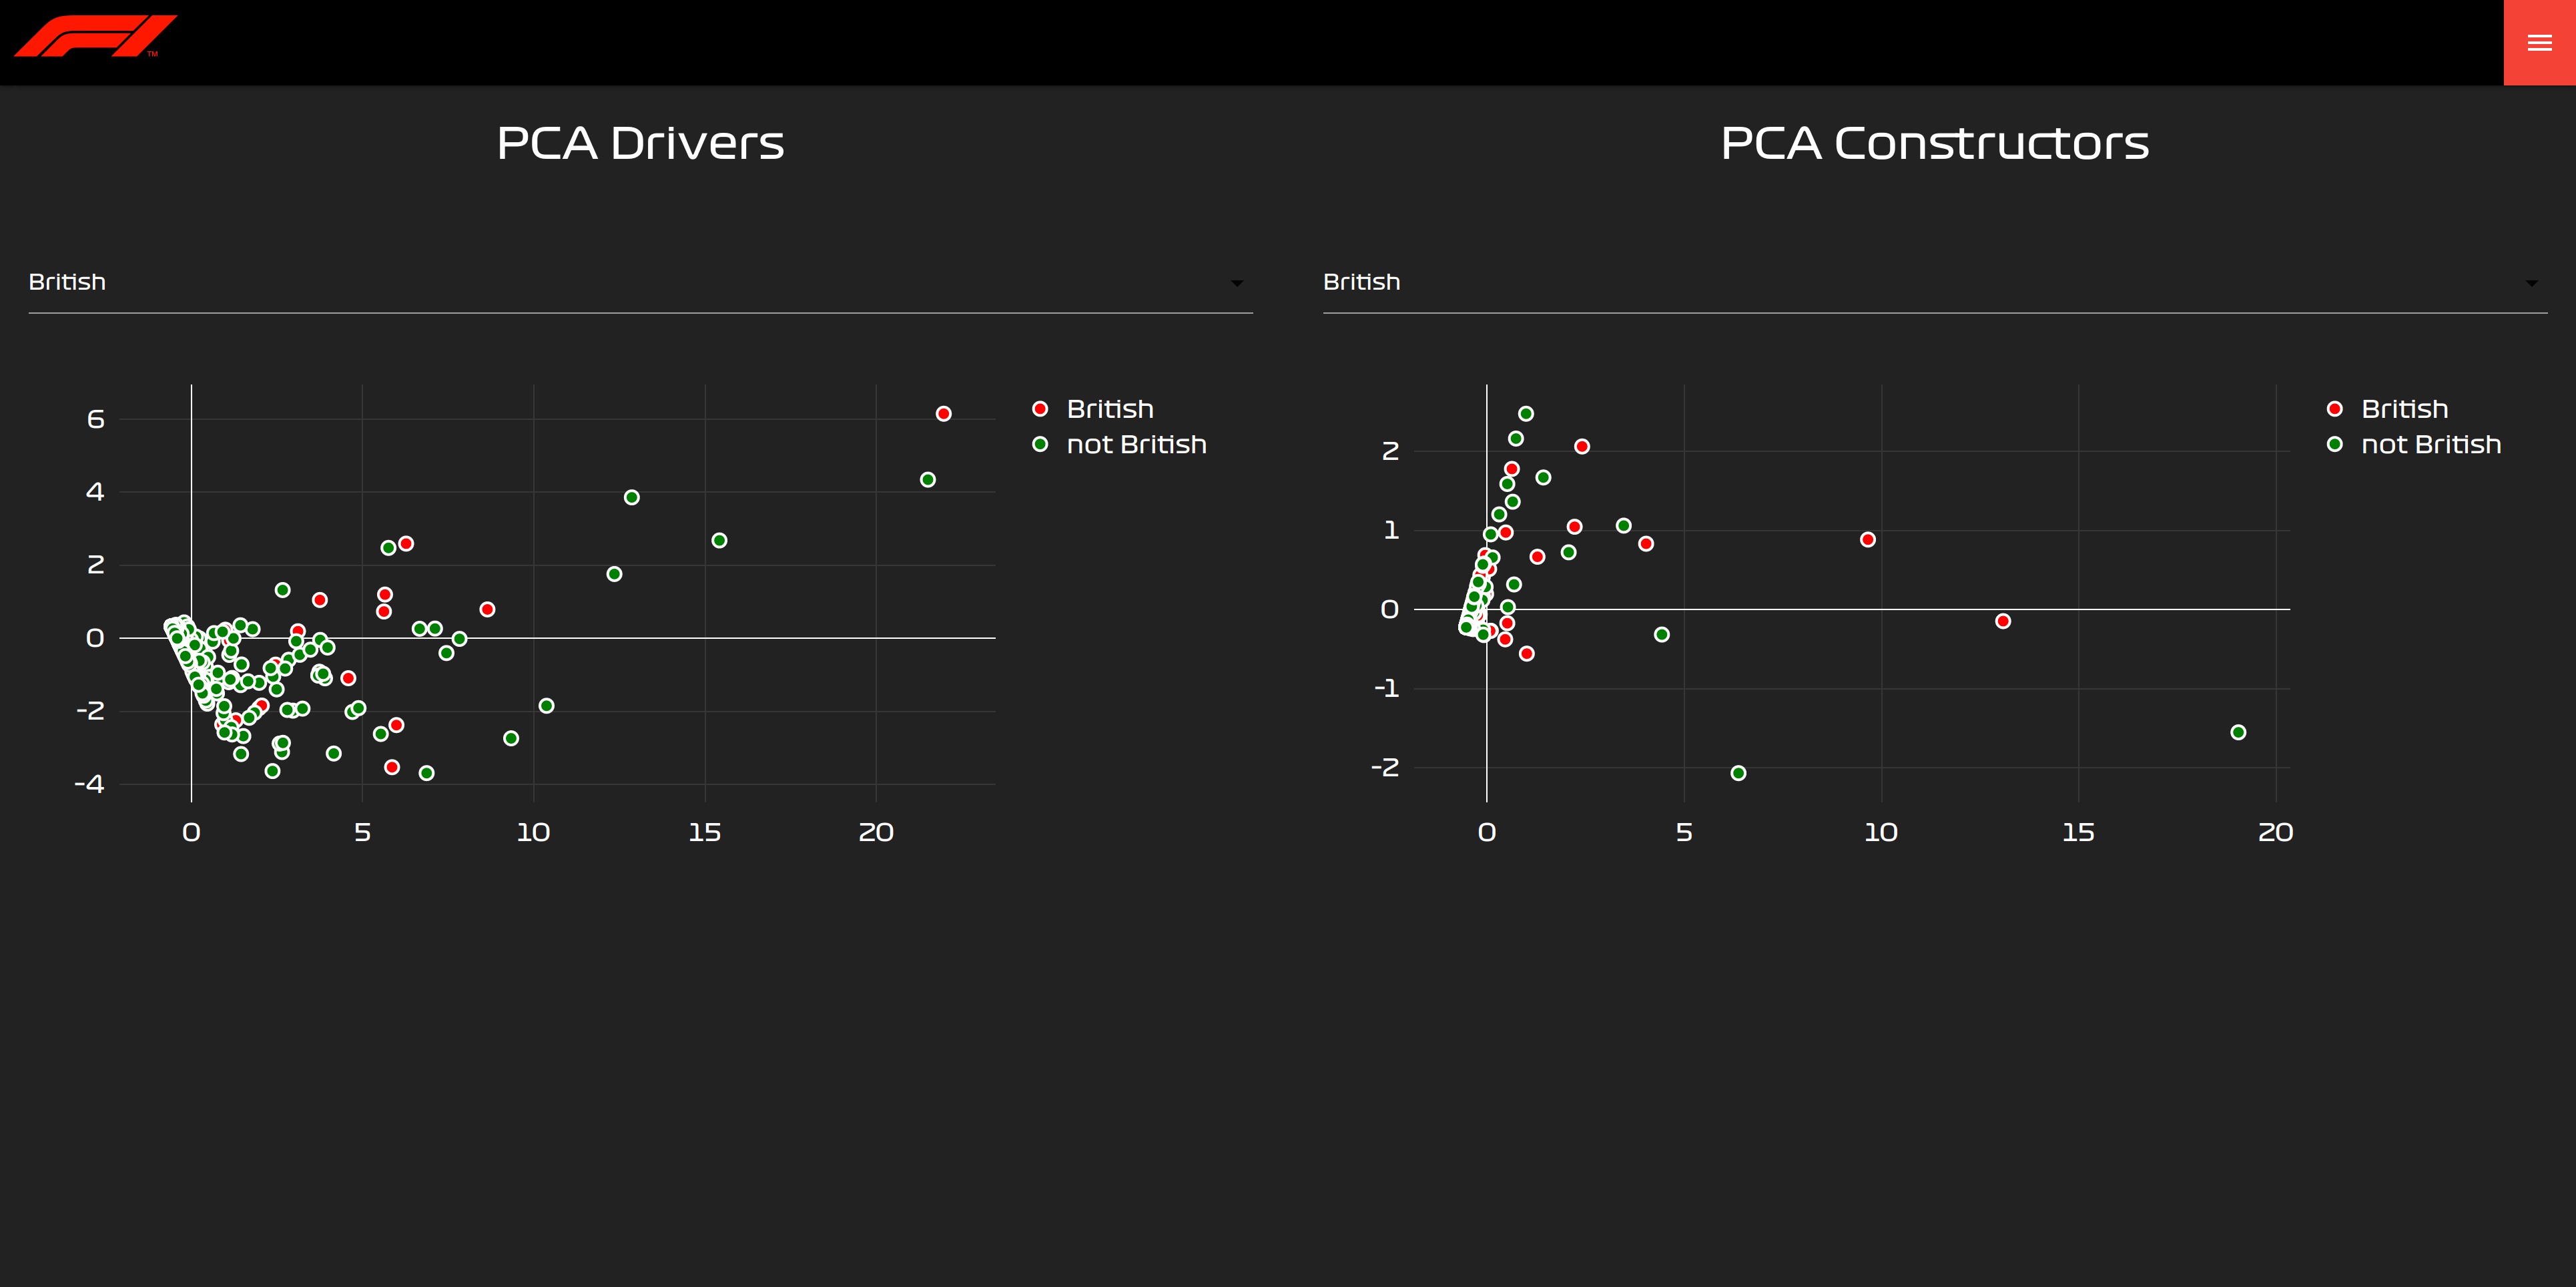
\includegraphics[width=\columnwidth]{correlations}
	\captionof{figure}{Correlations view}
\end{center}
This view is designed to show if there is a correlation between a specific nationality (selected by the user) and some statistics about the drivers and/or the constructors with that nationality. The view is divided into two sub-views: one for the drivers and one for the constructors. The user is able to select two different nationalities for the drivers and constructors using two different selectors. The result is plotted in the form of a scatter plot. In this two scatter plots the red point represents the elements of the nationality selected by the user while the green points represent the elements belonging to all the other nationalities. More details about the statistics that are taken into consideration are given in the analysis section.

\subsection{Times update view}
\begin{center}
	\centering
	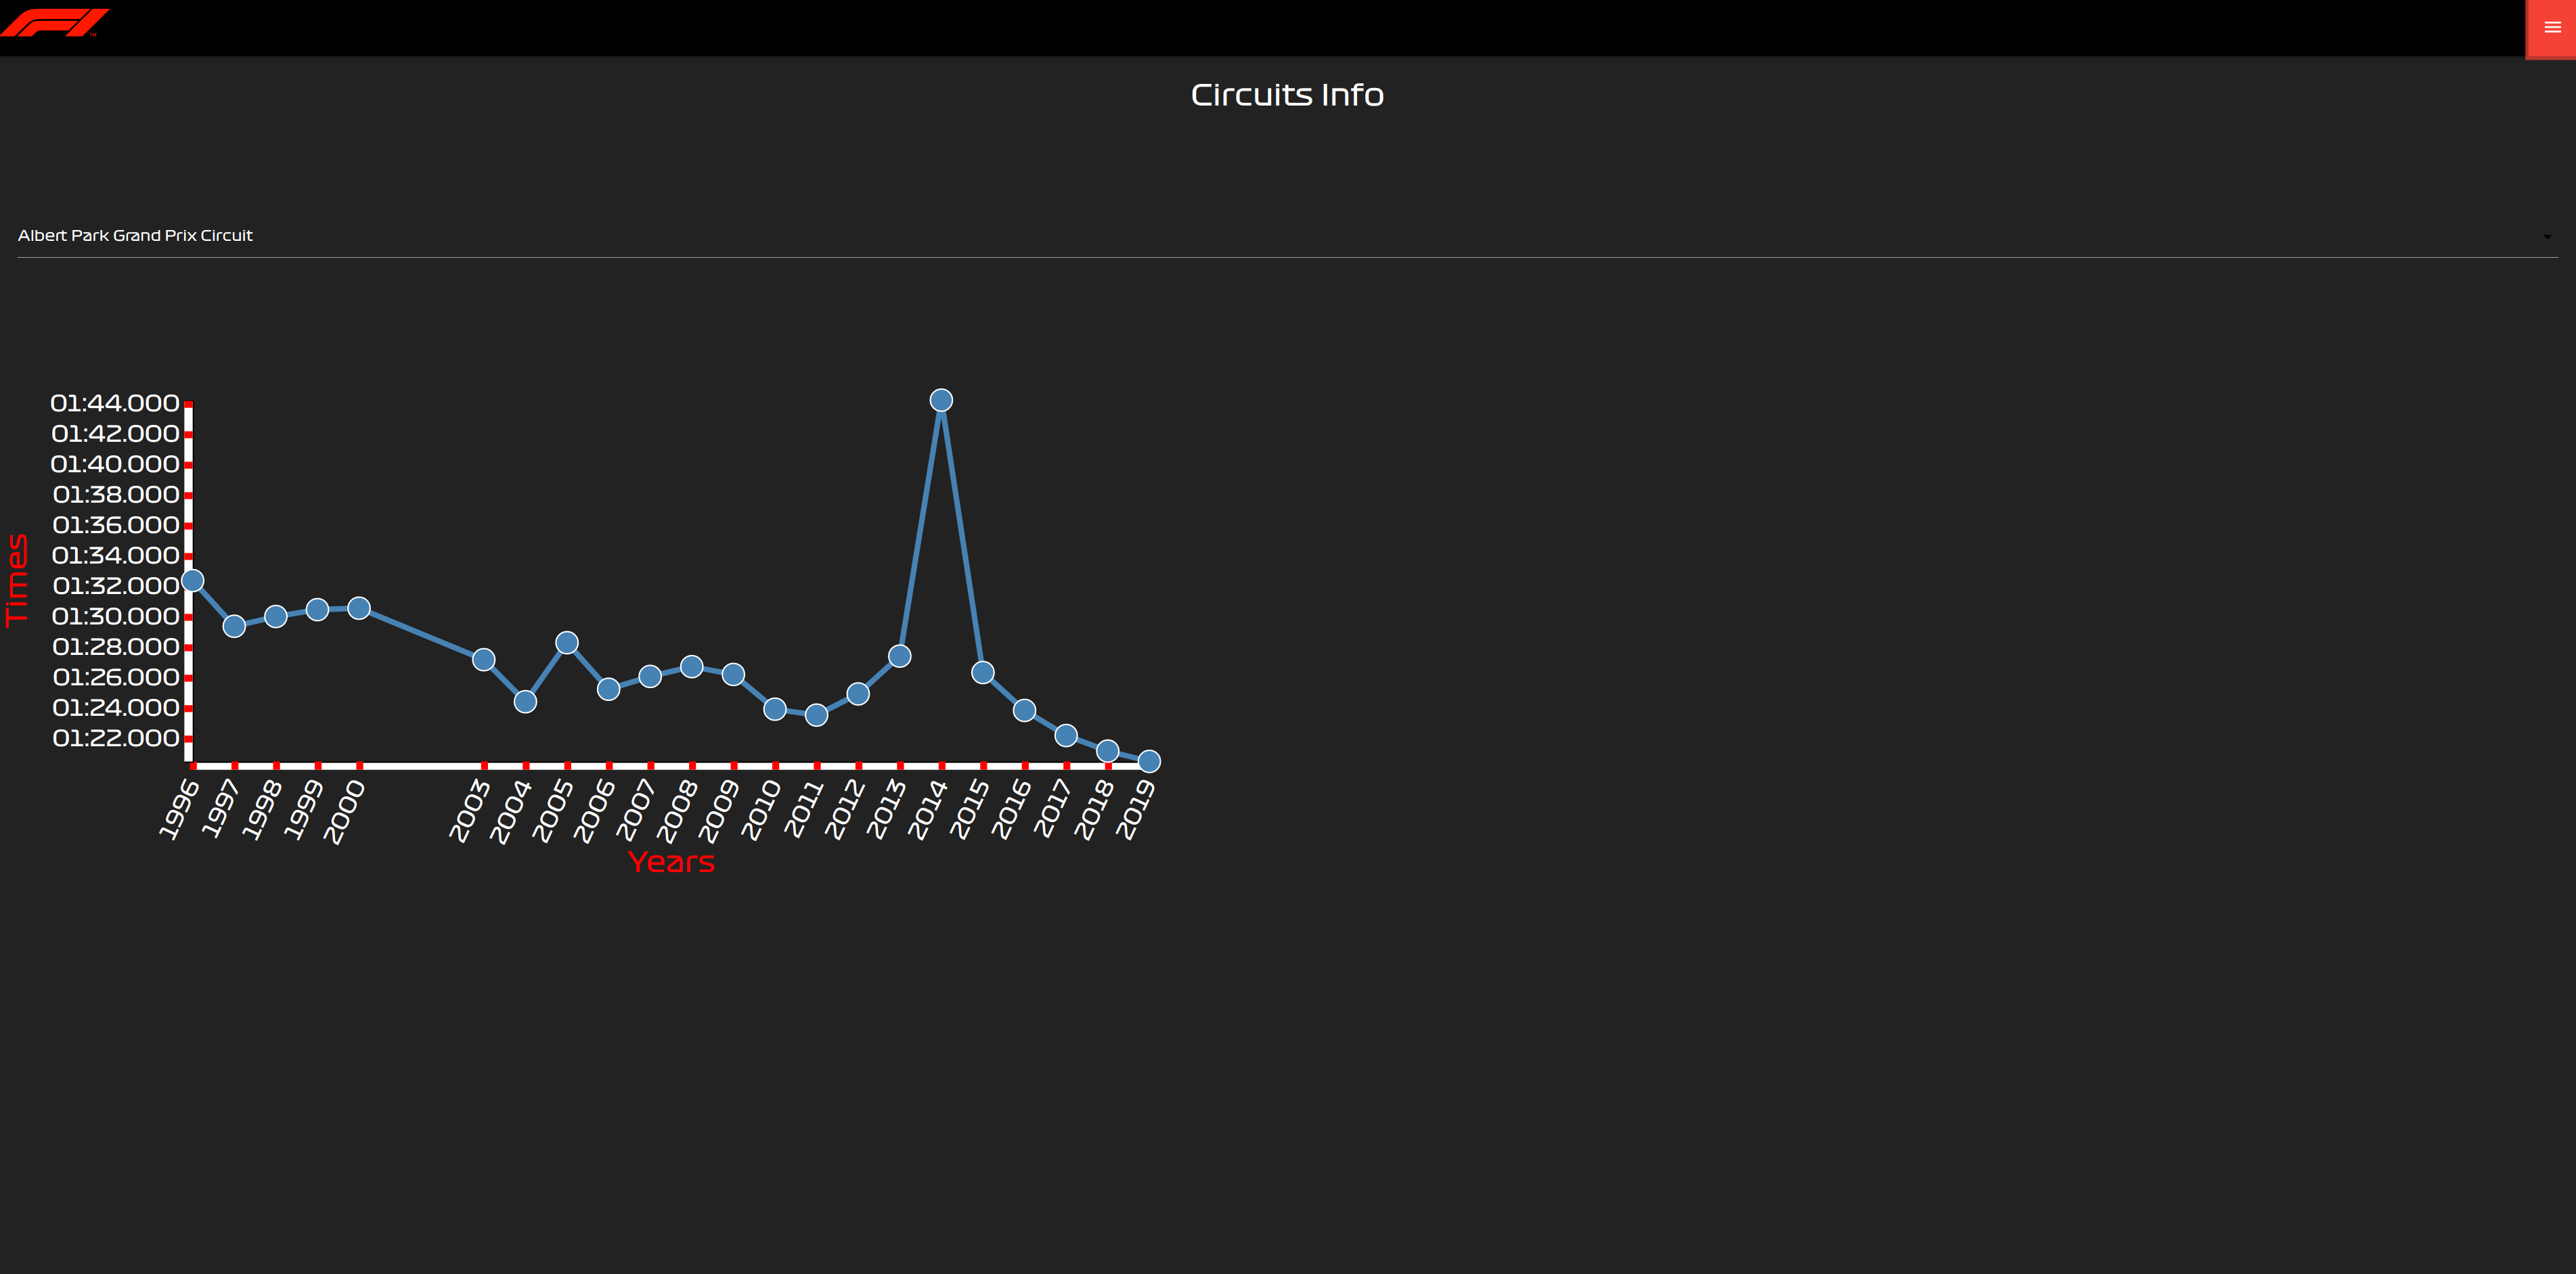
\includegraphics[width=\columnwidth]{timesupdate}
	\captionof{figure}{Times update view}
\end{center}
This last view shows the evolution of the lap times during the years for each circuit. The user can select one of the proposed circuits from the selector and then the scatter
plot will be updated. The lap times that are considered for creating this view are the pole position times for each Grand Prix over the years, so the fastest time
recorded during the qualifyings. Further informations about the selection of this lap time are provided in the Analytics section. On the x axis there are the years for which the
best lap time is available while the y-axis shows the times at intervals of different frequencies (the frequency depends on the number of different lap times for each year that
we have for each circuit).

\section{Analytics}
This section is more focused on data analysis and how to obtain, starting from the dataset, the views described above.\\
Most of the views are produced by manipulating the dataset in different ways starting from an input given by the user. This manipulation is done using the d3.js \cite{D3} library,
since it allows to do operations easily on .csv files and using Python 3 (in particular the pandas \cite{Pandas} and scikit-learn libraries \cite{Scikit-learn}) 
for analyse the correlation between nationality and number of wins/podiums. Most of the operations are characterized by a \texttt{JOIN} operation between the tables of the 
dataset and a subsequent \texttt{SELECT} operation over the desired attributes, in some cases with a \texttt{GROUP BY}.\\
An example could be the map in the main view: in this case we are interested in the circuits where there was at least one race during the year selected by the user. So, first
of all we make a \texttt{JOIN} between the two tables races and circuits over the attribute \texttt{circuitId} \texttt{WHERE} the year in which the race was run is equal to the
one selected by the user and then we \texttt{SELECT} the name of the circuits together with the corresponding country name and the name of the races. In SQL this query is like the
following:
\begin{itemize}
	\item \texttt{SELECT c.name, c.country, r.name}
	\item \texttt{FROM circuits c, races r}
	\item \texttt{WHERE c.circuitId == r.circuitId AND r.year == y}
\end{itemize}
where \texttt{y} is the year selected by the user.
At this point we are interested in two main values: the country in which the race was run and, in order to put the red circle on the map, the coordinates of the circuit. In order to
highlight in blue the country on the map, for each country we check if its name is into the set of country names resulting from the query described before. To add the red point
at the coordinates of the circuit we check, for each circuit, if the \texttt{circuitId} attribute is into the set of ids resulting from the previous query and then we take the
corresponding coordinates.\\
The Correlations View is based, as the name suggests, on the concept of correlation between attributes. In order to find if there is this correlation between attributes we have
decided to use the PCA algorithm, that is a statistical procedure that allows to summarize the information content in large data tables by means of a smaller set of “summary indices” 
that can be more easily visualized and analysed. In our case we have used PCA to check if there is a correlation between a nationality (selected by the user) and a set of features:
the number of victories, the number of podiums, the number of attendances and the number of pole positions done by a driver/constructor. The computation of PCA is done using Python 3 
and in particular using the implementation provided by the scikit-learn library \cite{Scikit-learn}. The idea is the following: if \texttt{n} is the nationality selected by the user 
then we create a new dataset in which we divide the drivers/constructors with respect to their nationality using the following binary classification: \texttt{n} vs non-\texttt{n}. 
Each row of this new dataset is composed by the following fields: number of victories, number of podiums, number of attendances and number of pole positions. Once done this we compute
PCA over this dataset performing the following three steps:
\begin{enumerate}
	\item Separate the labels (\texttt{n} and non-\texttt{n}) from the features
	\item Standardize the features (such that the variance of the data is 1 while their mean is 0)
	\item Perform the dimensionality reduction using the PCA algorithm (the data are projected on a 2D space)
\end{enumerate}
Since the user can select different nationalities through a selector, we decided to deploy the script that runs PCA on Heroku\cite{Heroku}, creating a simple server with Flask\cite{Flask}.
The resulting dataset is plotted using d3.js \cite{D3}.\\
As said in the previous section, the Times Update View is characterized by the evolution of the best lap times for each circuit selected by the user. A key point of this view is how to 
compute this best lap times. Since during Formula 1 history in addition to technology changes there have also been changes in the race regulations (such as changes applied to pit stop
rules) we have decided to take as best time for each circuit and each year the time of the pole position, so the fastest lap time registered during the qualifying of the race.
In the current regulation, the qualifying is divided into three phases: Q1, Q2 and Q3; the pole position is the fastest lap of the Q3 phase. But, by exploring the dataset, we have found
that there are some qualifyings for which one of the phases is not available (or no one of the phases; in this case obviously the race is not considered) so the fastest lap time is chosen
with the following criterion: if Q3 is not available the fastest lap time is the one registered during Q2; if Q2 is not available the fastest lap time is the one registered during
the Q1 phase.

\section{Future Works}
As the dataset provides a lot of data, it's possible to add more views to the application. We have in mind to add an interface that allows you to compare the statistics of the various 
drivers (e.g. number of wins, number of podiums, number of poles, etc.). The same could be done for constructors. Another interesting thing we would like to do is to have a projection of the remaining part of the current season considering both the races already raced in that season and the results obtained by the various drivers in previous seasons.

\section{Conclusion}
The project is useful to be able to retrace the history of Formula 1 easily, through intuitive graphics and a "sports" interface. The application could be used for different purposes,
for example by analysing the times over the years it is possible to guess how the technology or the skill of the pilots has progressed.
Learning how to use the framework is very simple, as we have chosen to use immediate and easily interpretable graphics. 

\clearpage

\twocolumn[{
	\renewcommand\twocolumn[1][]{#1}
	\begin{thebibliography}{100} 
		\bibitem{D3} Data-Driven Documents: \href{https://d3js.org/}{https://d3js.org/}
		
		\bibitem{HistoryOfF1} The history of Formula 1: \href{https://f1.bitmetric.nl/formula.html}{https://f1.bitmetric.nl/formula.html}
		
		\bibitem{Dataset} Ergast Developer API: \href{http://ergast.com/mrd/}{http://ergast.com/mrd/}
		
		\bibitem{Plotly} Plotly JavaScript Open Source Graphing Library: \href{https://plot.ly/javascript/}{https://plot.ly/javascript/}
		
		\bibitem{Pandas} Pandas library: \href{https://pandas.pydata.org/}{https://pandas.pydata.org/}
		
		\bibitem{Scikit-learn} Scikit-learn library: \href{https://scikit-learn.org/stable/}{https://scikit-learn.org/stable/}
		
		\bibitem{Heroku} Heroku: \href{https://www.heroku.com/}{https://www.heroku.com/}
		
		\bibitem{Flask} Flask: \href{https://flask.palletsprojects.com/en/1.1.x/}{https://flask.palletsprojects.com/en/1.1.x/}
	\end{thebibliography}
}]
\end{document}
